\subsection{MarineCity 3D Benchmark Protocol}
\label{sec:marinecity_3d_protocol}

This section reports the current MarineCity 3D/reasoner protocol and the
verified real-Cesium smoke-test artifacts. We do not present the smoke test as a
full benchmark result: it validates scene loading, multi-UAV capture,
SAFR-YOLO EvidenceToken export, 3D evidence grouping, and AeroGraph Reasoner
interface wiring. A 49-prompt AeroGraph schema-check record is available for the
current prompt pack, while external OpenAI/ChatGPT/local-provider replication is
reported separately as supplementary validation before any stronger final
reasoning claim.

The scene is centered on the Haeundae MarineCity region and is constructed in
Isaac Sim with Cesium geospatial context. The current verified smoke test uses
three UAV views over the saved real-Cesium \texttt{uavmarine.usd} stage. The UAV
camera altitude band is fixed to 140--160 m for the current protocol
(the latest viewer160 recapture uses 140/150/160 m for UAV~1/2/3 across
S0--S2), which is logged separately from the Cesium georeference height. Each UAV exports
RGB/depth-like capture artifacts, camera metadata, pose hints, and timestamp
fields. Vehicles and pedestrian-like small objects are placed from the detector
class vocabulary so that the 2D SAFR-YOLO output can be converted into
structured EvidenceTokens for the 3D graph and \textbf{AeroGraph Reasoner}.
The current actor-layer audit confirms six VisDrone-derived object cards
(vehicle classes plus pedestrian/person actors), three UAV markers, and three
UAV camera prims on the real-Cesium stage without synthetic city replacement.
The current SAFR-YOLO smoke runs produce detector EvidenceTokens for cars,
buses, vans, and pedestrians from the UAV views. The latest integration audit
reports 128 detector tokens over the three scenarios at the diagnostic
confidence setting, including 24 pedestrian tokens. The compact system table
below keeps the deterministic reasoner subset separate from this larger
detector aggregate, because the table is intended as pipeline validation rather
than as a final class-balanced quantitative benchmark.

The supplementary material summarizes the real-Cesium capture source now used
for the 3D/reasoner handoff. We intentionally report this as capture evidence
rather than as a full neural reconstruction benchmark. We additionally run
short Nerfstudio runner-family smoke experiments
on the exported MarineCity views to verify that neural 3D methods can be
trained and evaluated on the scene. The current verified rows cover Nerfacto,
Instant-NGP, and a Splatfacto/3DGS-style runner under the same sparse
real-Cesium capture split. These rows are system-executability evidence rather
than a final optimized 3D benchmark; longer validation is kept as an optional
late-stage improvement.
To verify that the captures are usable before installing the upstream neural
3D runners, we also export a NeRF-style \texttt{transforms.json} package and a
depth-fused colored point-cloud smoke artifact from the same nine
real-Cesium views. This point cloud is used only as a geometry handoff sanity
check in the supplementary material; it is not reported as a neural
completion/reconstruction result.

We also export the real-Cesium detector outputs into a cross-view evidence graph
for the current smoke protocol. The graph builder consumes 23 SAFR-YOLO
EvidenceTokens from the three-scenario, three-UAV capture, performs a
camera-metadata-based approximate ray projection, and groups them into 13
object hypotheses. Five hypotheses receive multi-view support, while the graph
records 23 support edges, 4 conflict edges, and 20 missing-evidence edges for
downstream ambiguity handling. This is a protocol validation of evidence
association and uncertainty routing, not a completed metric 3D reconstruction.
The detailed graph table is placed in the supplementary material.

The protocol reserves train, validation, and held-out unseen-angle test splits
with multiple UAV viewpoints, including nadir, front-oblique, side, rear-oblique,
right-oblique, and left-oblique cameras. The held-out split emphasizes
unseen viewpoints so that the reconstruction and reasoning components are tested
on viewpoint generalization rather than memorized camera poses. The first smoke
test focuses on a small number of manually verified scenes rather than a
large synthetic dataset claim.

\paragraph{3D and reasoner evaluation slots.}
The validated smoke test already runs: (1) SAFR-YOLO on each UAV view, (2)
detector outputs as EvidenceTokens, (3) token grouping into 3D evidence
hypotheses, and (4) \textbf{AeroGraph Reasoner}, the drone-specialized
graph-grounded LLM/VLM reasoner, to propose verified class/action decisions
under a safety-verifier schema. The current system-smoke reasoner provider is a
deterministic rule-based verifier for system validation, not a final
external-provider LLM/VLM result. A separate 49-prompt AeroGraph validation record has valid
schema-checked JSON outputs and is kept in the supplementary validation record
until an OpenAI/ChatGPT/local provider replication is imported. For 3D
completion, Table~\ref{tab:marinecity_3d_completion_results} now contains three
completed smoke rows on the real-Cesium capture package: Nerfacto,
Instant-NGP, and a Splatfacto/3DGS-style runner. These rows demonstrate that the
neural-3D handoff is executable across multiple runner families; they are not
claimed as a full optimized 3D benchmark until longer validation and cleaner
reconstruction captures are completed.
Table~\ref{tab:marinecity_system_smoke} summarizes the completed smoke-test
artifacts. The current AeroGraph prompt/schema validation details
remain in the supplementary material as validation support rather than as the
headline system result.

\begin{table}[t]
\centering
\scriptsize
\setlength{\tabcolsep}{3pt}
\caption{MarineCity neural 3D completion smoke metrics on held-out real-Cesium
MarineCity views. Only completed runner rows are included; these rows verify
runner-family execution rather than claim a final optimized benchmark.}
\label{tab:marinecity_3d_completion_results}
% Auto-generated by scripts/build_marinecity_3d_results_table.py
% Pending-safe: placeholder/dry-run rows are intentionally excluded.
\begin{tabular}{lrrrrrl}
\toprule
Method & PSNR$\uparrow$ & SSIM$\uparrow$ & LPIPS$\downarrow$ & FPS$\uparrow$ & Time (min)$\downarrow$ & Status \\
\midrule
Nerfacto (torch smoke) & 22.73 & 0.938 & 0.072 & 0.59 & -- & complete\_native\_nerfacto\_torch\_split067\_noapp\_8k \\
3D Gaussian Splatting & 19.68 & 0.807 & 0.170 & 4.56 & -- & complete\_native\_splatfacto\_split067\_5k \\
\bottomrule
\end{tabular}

\end{table}

\begin{table}[t]
\centering
\caption{MarineCity multi-UAV system smoke-test results. The current reasoner provider is a deterministic AeroGraph mock; non-mock LLM/VLM validation is marked as pending for the final system study.}
\label{tab:marinecity_system_smoke}
\resizebox{\linewidth}{!}{%
\begin{tabular}{lrrrrll}
\toprule
Scenario & UAV views & Evidence tokens & 3D hypotheses & Re-observe & Detected classes & Provider \\
\midrule
S0 locked MarineCity ROI & 3 & 19 & 13 & 13 & car=14, bus=5 & mock\_symbolic\_aerograph \\
S1 adjacent/overlapping objects & 3 & 25 & 17 & 17 & bus=7, car=17, pedestrian=1 & mock\_symbolic\_aerograph \\
S2 coastline multi-view ambiguity & 3 & 29 & 19 & 19 & bus=6, car=20, pedestrian=3 & mock\_symbolic\_aerograph \\
\bottomrule
\end{tabular}%
}
\end{table}


\begin{figure}[t]
\centering
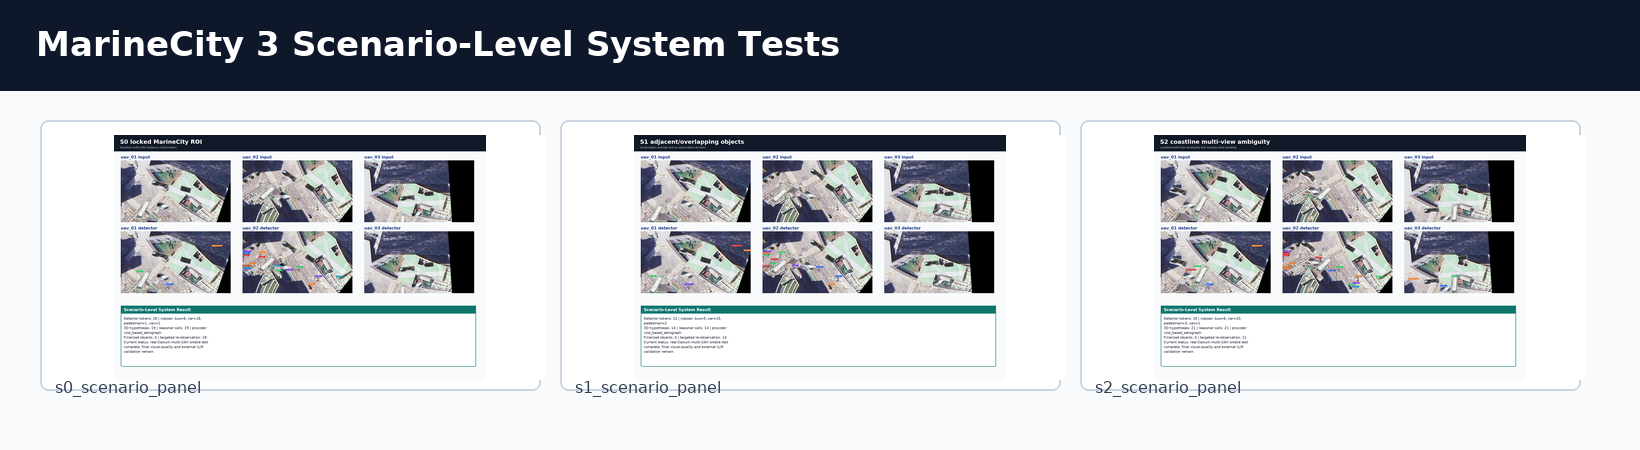
\includegraphics[width=0.95\linewidth]{figures/results/marinecity_system/contact_sheet_3_scenarios.png}
\caption{Representative qualitative MarineCity system-smoke evidence. The
panels show real-Cesium UAV views, detector overlays, and scenario-level
evidence used to build the cross-view graph. This figure complements the
quantitative detector and 3D smoke tables in the main paper.}
\label{fig:marinecity_main_qualitative}
\end{figure}

\paragraph{Reporting rule.}
Unverified provider outputs and command-contract checks are kept outside the
headline claim. The main paper reports the verified
real-Cesium capture, detector-token, and smoke-test tables now, but reserves
final external-provider LLM/VLM and 3D completion claims until replicated
provider runs and completion/restoration experiments are validated.
